\section{Cliente}
Oltre alle funzionalità presenti come ospite, un cliente può effettuare 
le seguenti azioni:
\begin{itemize}
    \item Accedere alla propria area personale (My Area)
    \item Aggiungere ristoranti ai preferiti
    \item Scrivere recensioni sui ristoranti
\end{itemize}

\subsection{Area Privata Cliente}
Premendo sul pulsante \emph{My Area} in alto a destra nella schermata 
di ricerca (Figura~\ref{fig:search}), l'utente accede alla propria area personale.\\
In questa schermata l'utente può visualizzare:
\begin{itemize}
    \item Quanti ristoranti ha aggiunto ai preferiti in alto a sinistra
    \item Qual è il punteggio medio delle recensioni scritte a fianco del numero di ristoranti preferiti
    \item Il numero di recensioni scritte a fianco del loro punteggio medio
    \item Elenco dei ristoranti preferiti a sinistra
    \item Elenco delle recensioni scritte a destra
    \item In alto a destra un pulsante \emph{Logout} per tornare alla schermata di login (Figura~\ref{fig:login})
    \item In alto a destra, a fianco del pulsante di Logout, 
    un pulsante \emph{Back to Search} per tornare alla 
    schermata di ricerca (Figura~\ref{fig:search})
\end{itemize}

\begin{figure}[H]
    \centering
    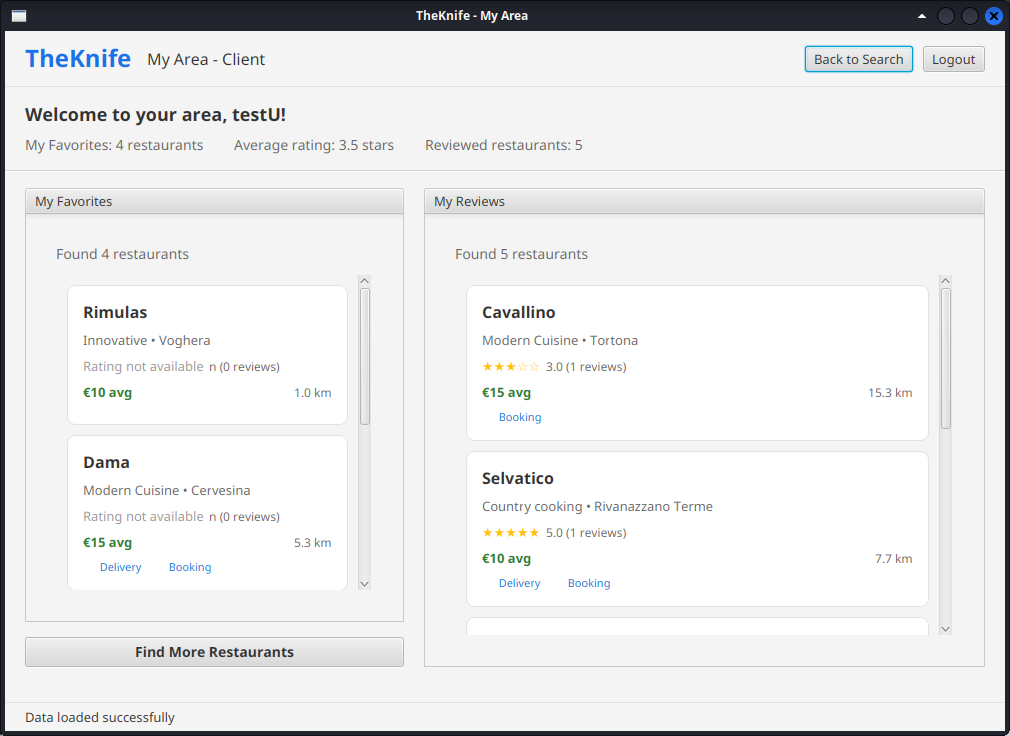
\includegraphics[width=0.8\textwidth]{images/myarea-client.png}
    \caption{Area Privata Cliente}
    \label{fig:myarea-client}
\end{figure}
Da questa schermata l'utente può agevolmente gestire i suoi ristoranti 
preferiti e le recensioni scritte modificandoli o cancellandoli.
\paragraph{Nota}
Le modifiche effettuate nella propria area 
personale non sono immediatamente visibili. Occorre uscire 
dalla propria area personale e rientrare per visualizzare 
le modifiche apportate.

\subsection{Preferiti}
Dalla vista del dettaglio del ristorante (Figura~\ref{fig:restaurant}), 
raggiungibile premendo sul nome di un ristorante, l'utente può 
aggiungere il ristorante ai preferiti premendo il pulsante 
\emph{Add to Favourites}. Una volta premuto il pulsante il ristorante 
verrà automaticamente aggiunto alla lista dei preferiti e comparirà
nella propria area personale (Figura~\ref{fig:myarea-client}) la 
prossima volta che si premerà il pulsante \emph{My Area}.

\subsection{Recensioni}
Dalla vista del dettaglio del ristorante (Figura~\ref{fig:restaurant})
l'utente può scrivere una recensione premendo il pulsante 
\emph{Write a Review}. 
Una volta premuto il pulsante comparirà una schermata per scrivere 
la propria recensione.\\
Selezionare un punteggio da 1 a 5 premendo sulla stella corrispondente
il punteggio che si desidera assegnare.
Se lo si desidera, scrivere un commento nella casella di testo.
Il commento è facoltativo, ma è consigliato per rendere la recensione
più utile agli altri utenti.\\
Le recensioni possono essere modificate o cancellate in qualsiasi 
momento dalla propria area personale (Figura~\ref{fig:myarea-client}).
\begin{figure}[H]
    \centering
    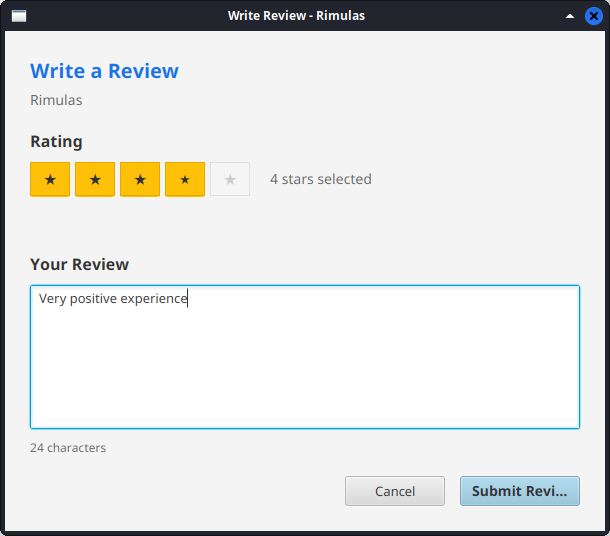
\includegraphics[width=0.8\textwidth]{images/review.png}
    \caption{Schermata di scrittura recensione}
    \label{fig:review}
\end{figure}
\paragraph{Nota}
Il commendo non può eccederei i 255 caratteri.
